\chapter{Package Diagramm}
Wir haben uns ein Package Diagramm überlegt, welches uns ermöglichen soll möglichst flexibel Packages zu ersetzen/hinzufügen, ohne dass die Hauptlogik (enthalten im "Business Layer" und im "Common Layer") verändert werden muss.
\begin{figure}[H]
\centering
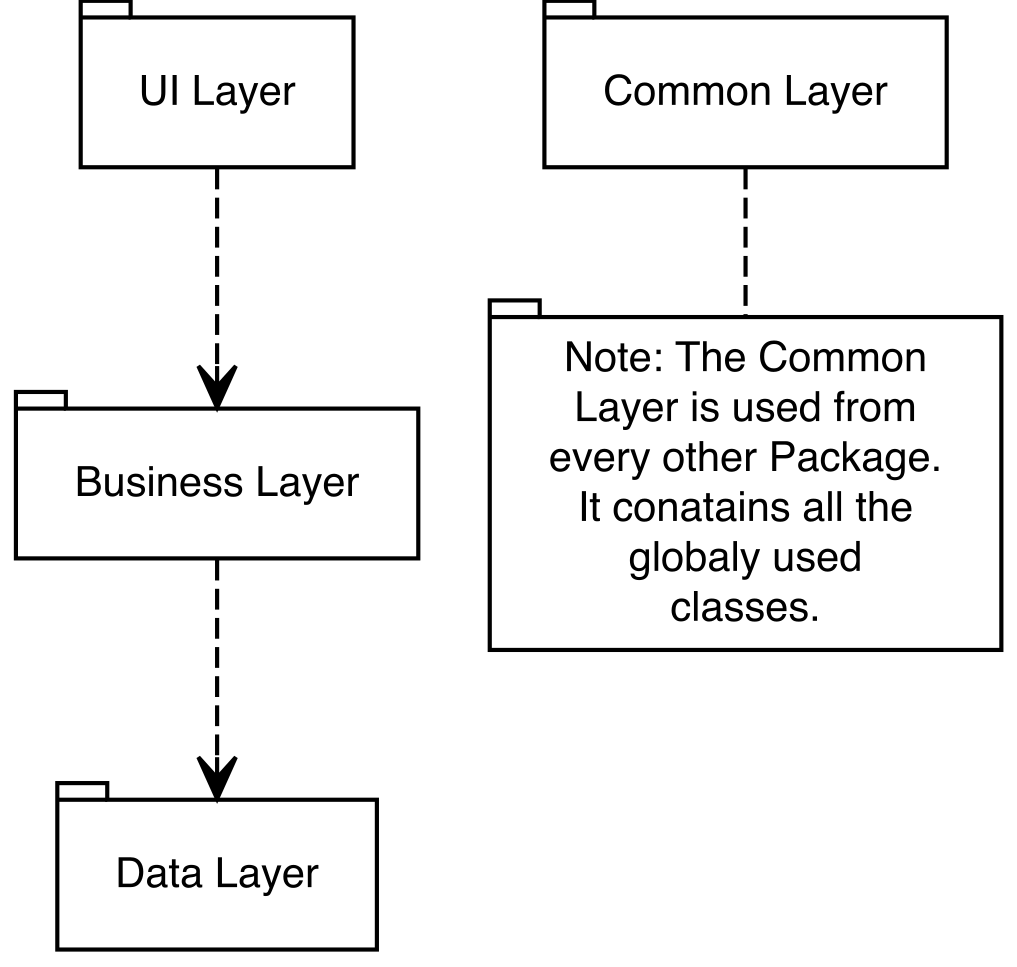
\includegraphics[width=1\textwidth]{../PackageDiagramm/PackageDiagramm.png}
\caption{Package Diagramm}
\end{figure}

\section{UI Layer}
Im UI Layer wird die ganze UI Logik gehandelt, es wird das "Business Layer" und das "Common Layer" Package verwendet. Ziel dabei ist es, falls ein neues oder zusätzliches UI erstellt werden soll, dass das Package möglichst einfach an die Kern Logik angebunden werden kann.

\section{Business Layer}
Im Business Layer wird die gesammte Logik der Applikation abgebildet.

\section{Data Layer}
Der Data Layer ist für die Speicherung und für das Abrufen von Daten zuständig.

\section{Common Layer}
Im Common Layer sind die Klassen bzw. Models enthalten die in allen anderen Packages verwendet werden. Z.B: die User Klasse oder die Challenge Klasse.

